\documentclass[a4paper,9pt]{extarticle}

%=========================================================
% PACKAGES
%=========================================================

\usepackage[
a4paper,
top=1.8cm,
bottom=1.5cm,
footskip=7mm,
left=1cm,
right=1cm,
headheight=14pt,
headsep=5mm
]{geometry}

\usepackage[T1]{fontenc}
\usepackage[utf8]{inputenc}
\usepackage[french]{babel}

\usepackage[sfdefault]{FiraSans}
\renewcommand{\familydefault}{\sfdefault}

\usepackage{multicol}
\setlength{\columnsep}{0.7cm}

\usepackage{amsmath,amssymb}
\usepackage{titlesec}
\usepackage{enumitem}

\usepackage{tcolorbox}
\tcbuselibrary{skins,breakable}

\usepackage{xcolor}
\usepackage{graphicx}
\usepackage{float}
\usepackage{tikz}

\usepackage{fancyhdr}
\usepackage[hidelinks]{hyperref}


%=========================================================
% PAGE SETTINGS
%=========================================================

\setlength{\parindent}{0pt}
\setlength{\parskip}{1.5pt}

\setlength{\abovedisplayskip}{4pt}
\setlength{\belowdisplayskip}{4pt}

\setlist[itemize]{
leftmargin=*,
itemsep=1pt,
topsep=1pt
}


%=========================================================
% COLORS
%=========================================================

\definecolor{Blue}{HTML}{E3F0FF}
\definecolor{Green}{HTML}{E3F7EA}
\definecolor{Pink}{HTML}{FFE5ED}
\definecolor{Orange}{HTML}{FFF0DC}
\definecolor{Purple}{HTML}{EEE7FF}
\definecolor{Yellow}{HTML}{FFFADB}

\definecolor{BlueTitle}{HTML}{285B8F}
\definecolor{GreenTitle}{HTML}{287052}
\definecolor{PinkTitle}{HTML}{A84063}
\definecolor{OrangeTitle}{HTML}{A96500}
\definecolor{PurpleTitle}{HTML}{6245A5}


%=========================================================
% HEADER
%=========================================================

\pagestyle{fancy}
\fancyhf{}

\fancyhead[L]{\small\textbf{Electronique I}}
\fancyhead[C]{\small Composants, Kirchhoff et simplifications}
\fancyhead[R]{\small Week 03 -- 21-27/09/2026}

\fancyfoot[C]{\small\href{https://github.com/AlphaXT38G/notes_ba5}{github.com/AlphaXT38G/notes\_ba5}}
\fancyfoot[R]{\small \thepage}

\renewcommand{\headrulewidth}{0.4pt}


%=========================================================
% TITLES
%=========================================================

\titleformat{\section}
{\large\bfseries\color{BlueTitle}}
{}{0pt}{}

\titlespacing{\section}
{0pt}{6pt}{3pt}


%=========================================================
% SEPARATOR
%=========================================================

\newcommand{\separator}{
\vspace{2pt}
\hrule
\vspace{3pt}
}


%=========================================================
% BOXES
%=========================================================

% DEFINITION - blue

\newtcolorbox{definition}{
enhanced,
breakable,
colback=Blue,
colframe=BlueTitle,
boxrule=0.7pt,
arc=0mm,
title=\textbf{Definition},
fonttitle=\bfseries
}


% IMPORTANT - pink

\newtcolorbox{important}{
enhanced,
breakable,
colback=Pink,
colframe=PinkTitle,
boxrule=0.7pt,
arc=0mm,
title=\textbf{Key idea},
fonttitle=\bfseries
}


% FORMULAS - green

\newtcolorbox{formula}{
enhanced,
breakable,
colback=Green,
colframe=GreenTitle,
boxrule=0.7pt,
arc=0mm,
title=\textbf{Key formulas},
fonttitle=\bfseries
}


% WARNING - orange

\newtcolorbox{warning}{
enhanced,
breakable,
colback=Orange,
colframe=OrangeTitle,
boxrule=0.7pt,
arc=0mm,
title=\textbf{Warning},
fonttitle=\bfseries
}


% EXAMPLE - purple

\newtcolorbox{example}{
enhanced,
breakable,
colback=Purple,
colframe=PurpleTitle,
boxrule=0.7pt,
arc=0mm,
title=\textbf{Example},
fonttitle=\bfseries
}


% SUMMARY - yellow

\newtcolorbox{summary}{
enhanced,
breakable,
colback=Yellow,
colframe=OrangeTitle,
boxrule=0.7pt,
arc=0mm,
title=\textbf{Summary},
fonttitle=\bfseries
}


%=========================================================
% DOCUMENT
%=========================================================

\begin{document}

\thispagestyle{fancy}

\footnotesize

\begin{multicols}{2}


%=========================================================
\section{Composants de base : la résistance}


\begin{center}

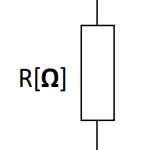
\includegraphics[
width=0.18\linewidth
]{../images/week03_01.png}

\end{center}


\begin{formula}

Si la source de \textbf{courant} est continue (valeur constante) :

\[
U = R\cdot I
\]

Si la source de \textbf{tension} est continue (valeur constante) :

\[
I = \frac{U}{R}
\]

où :

\begin{itemize}

\item $U$ : tension aux bornes de la résistance [V] ;

\item $I$ : courant qui la traverse [A] ;

\item $R$ : résistance [$\Omega$].

\end{itemize}

\end{formula}


%=========================================================
\section{Composants de base : le condensateur}


\begin{definition}

Un condensateur est un petit réservoir de charges électriques : il stocke de l'énergie en accumulant des charges sur ses deux plaques, comme un réservoir se remplit d'eau.

\end{definition}


\begin{center}

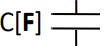
\includegraphics[
width=0.25\linewidth
]{../images/week03_02.png}

\end{center}


\begin{center}

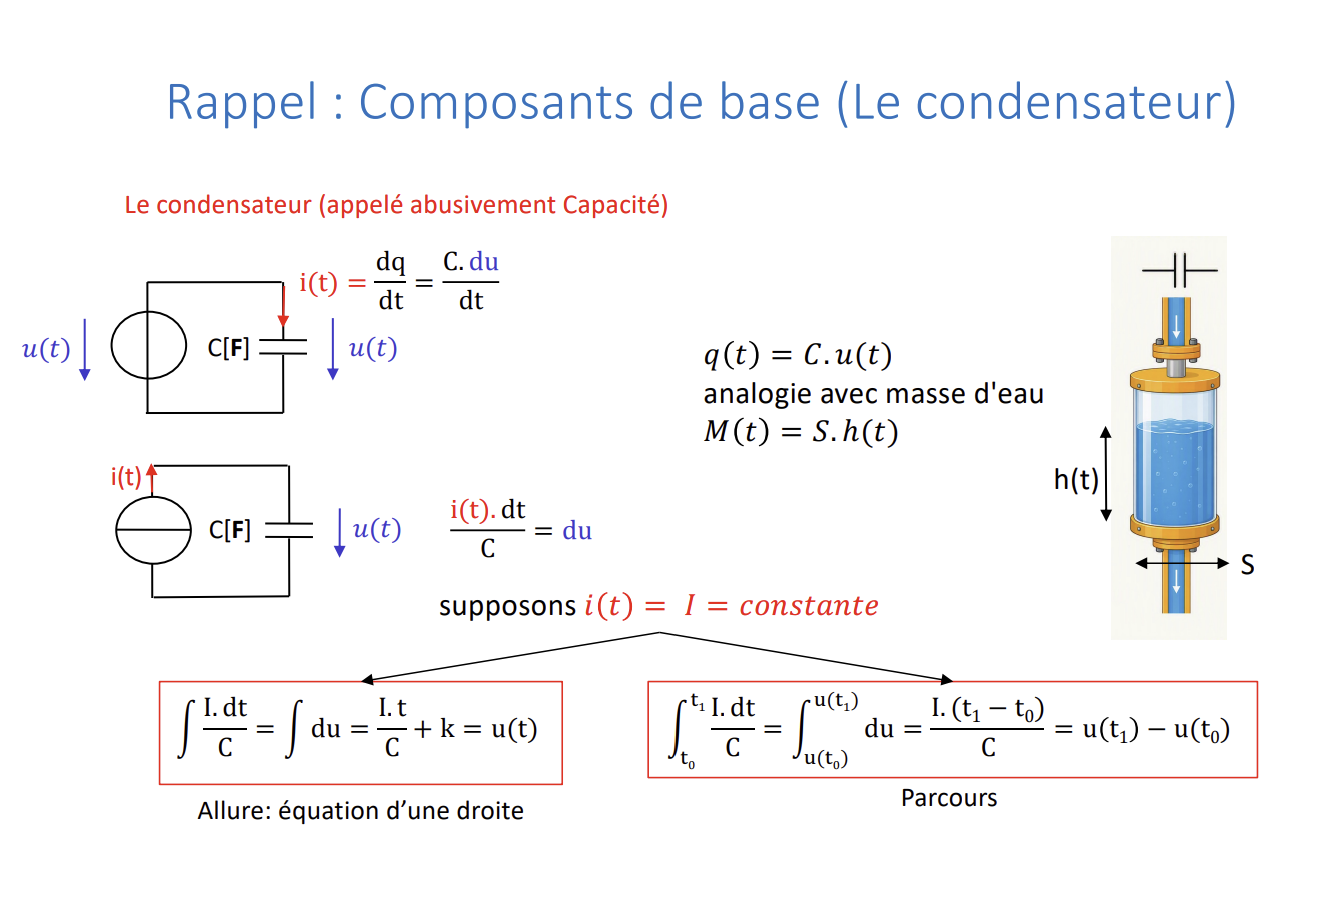
\includegraphics[
width=1.0\linewidth
]{../images/week03_03.png}

\end{center}


\begin{formula}

Avec une source de \textbf{tension} :

\[
i(t) = \frac{dq}{dt} = C\,\frac{du}{dt}
\qquad
q(t) = C\,u(t)
\]

avec $C$ la capacité du condensateur ; $q(t)$ est ici la charge du condensateur.

\vspace{3pt}

Avec une source de \textbf{courant} :

\[
du = \frac{i(t)\,dt}{C}
\]

On résout ici par une intégrale : si $i(t) = I$ est constant, c'est une constante dans le calcul intégral ; si le courant dépend de $t$, alors par exemple $i(t) = A\sin(\omega t)$.

\vspace{3pt}

où :

\begin{itemize}

\item $i(t)$ : courant qui traverse le condensateur [A] ;

\item $u(t)$ : tension aux bornes du condensateur [V] ;

\item $q(t)$ : charge stockée [C] (coulomb), $1\,\text{C} = 1\,\text{A}\cdot\text{s}$ ;

\item $C$ : capacité [F] (farad), $1\,\text{F} = 1\,\text{C}/\text{V}$ ;

\item $t$ : temps [s] ; $dq$, $du$, $dt$ : petites variations de $q$, $u$, $t$ ;

\item $A$ : amplitude du courant [A] ; $\omega$ : pulsation [rad/s] ;

\item $k$ : constante d'intégration [V] (la tension de départ).

\end{itemize}

\end{formula}


%=========================================================
\section{Composants de base : l'inductance}


\begin{definition}

Une inductance est une bobine de fil qui s'oppose aux changements du courant qui la traverse : elle stocke de l'énergie dans un champ magnétique, comme une roue lancée qui résiste quand on veut l'accélérer ou la freiner.

\end{definition}


\begin{center}

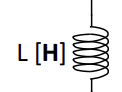
\includegraphics[
width=0.2\linewidth
]{../images/week03_04.png}

\end{center}


\begin{center}

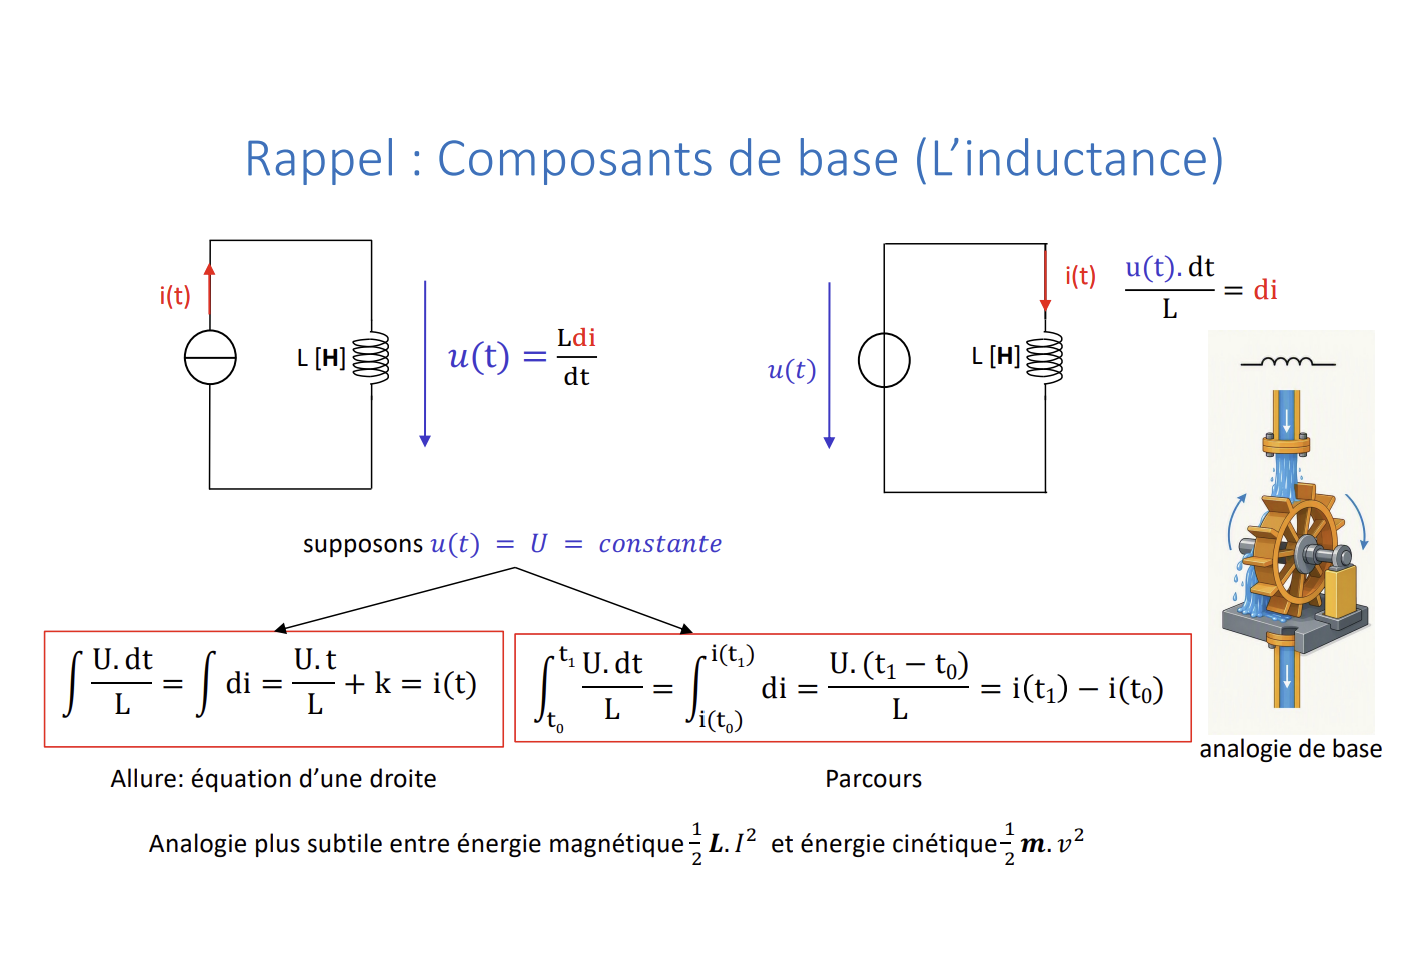
\includegraphics[
width=1.0\linewidth
]{../images/week03_05.png}

\end{center}


\begin{formula}

Avec une source de \textbf{courant} :

\[
u(t) = L\,\frac{di}{dt}
\]

Avec une source de \textbf{tension} :

\[
\frac{u(t)\,dt}{L} = di
\]

où :

\begin{itemize}

\item $u(t)$ : tension aux bornes de l'inductance [V] ;

\item $i(t)$ : courant qui la traverse [A] ;

\item $L$ : inductance [H] (henry), $1\,\text{H} = 1\,\text{V}\cdot\text{s}/\text{A}$ ;

\item $t$ : temps [s] ; $di$, $dt$ : petites variations de $i$ et $t$ ;

\item $k$ : constante d'intégration [A] (le courant de départ) ;

\item énergie magnétique $\frac{1}{2}L I^2$ [J], analogue à l'énergie cinétique $\frac{1}{2}m v^2$ ($m$ : masse [kg], $v$ : vitesse [m/s]).

\end{itemize}

\end{formula}


\textbf{Résumé des trois composants}

\begin{center}

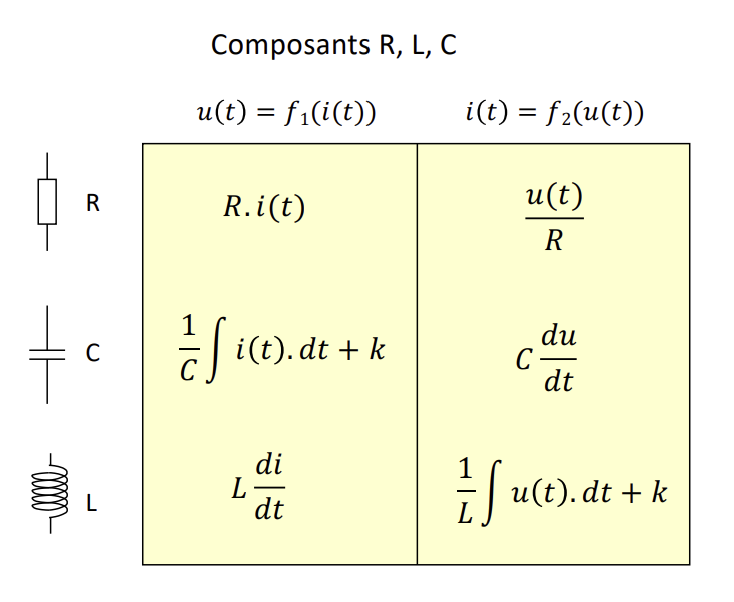
\includegraphics[
width=0.8\linewidth
]{../images/week03_06.png}

\end{center}


%=========================================================
\section{Lois de Kirchhoff : définitions}


\begin{definition}

Un circuit est composé de \textbf{segments} :

\begin{itemize}

\item ils portent des composants ;

\item ils se connectent entre eux.

\end{itemize}

On nomme les extrémités des segments : les \textbf{nœuds}.

\vspace{3pt}

\textbf{Nœud} : connexion entre deux segments au moins. Exemple : $A$ (2 segments) et $B$ (3 segments).

\textbf{Branche} : succession de segments connectés deux par deux. Exemple : $ABCD$.

\textbf{Maille} : parcours fermé, constitué de branches, ne passant qu'une seule fois par un nœud donné.

\end{definition}


%=========================================================
\section{Loi des mailles}


\begin{center}

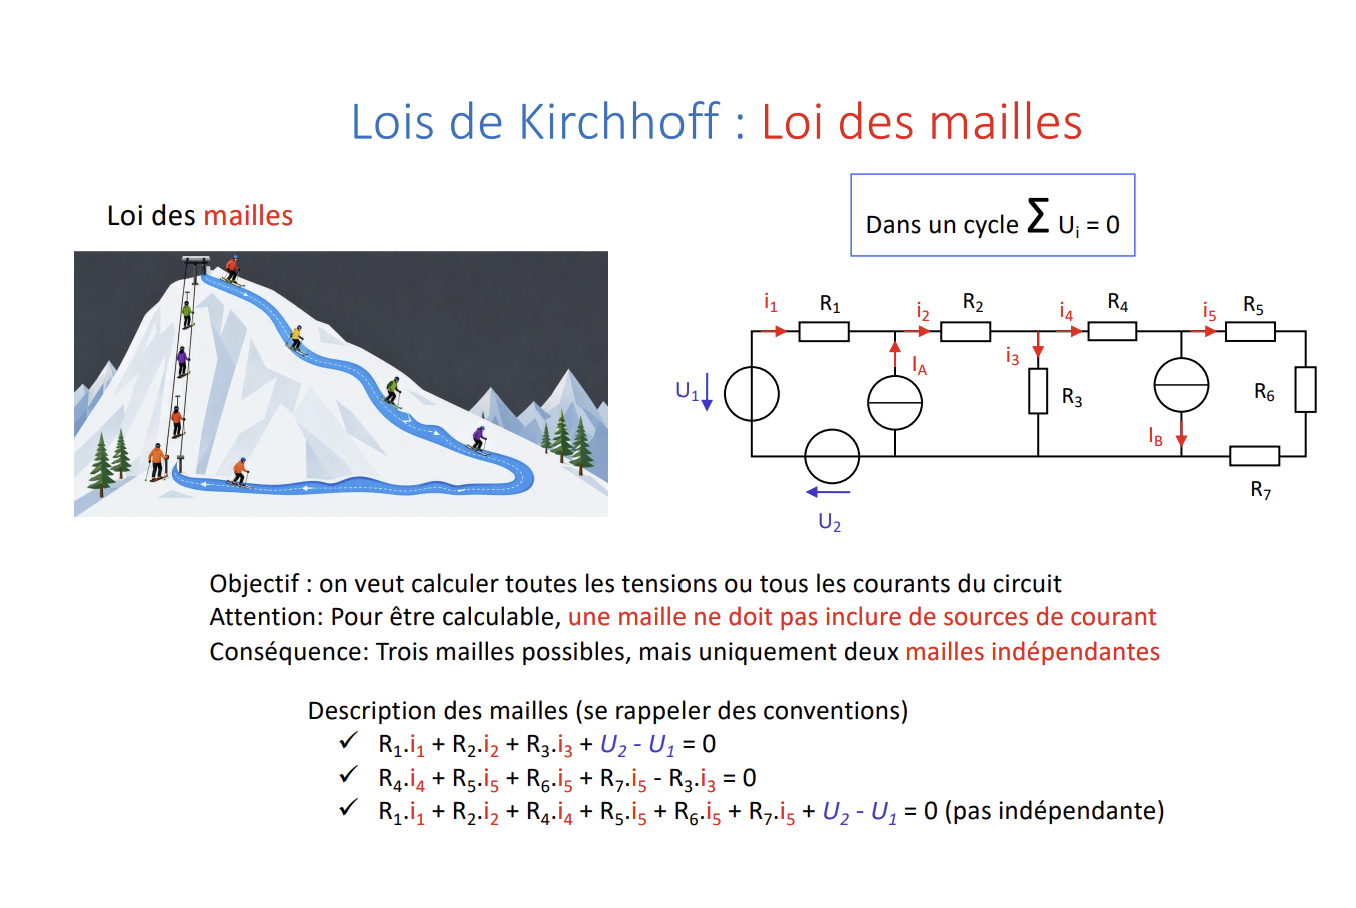
\includegraphics[
width=1.0\linewidth
]{../images/week03_07.png}

\end{center}


\begin{formula}

Dans un cycle (une maille) :

\[
\sum_i U_i = 0
\]

où $U_i$ : tension aux bornes du $i$-ème élément de la maille [V], comptée positive ou négative selon le sens de parcours (se rappeler des conventions).

\end{formula}


\textbf{Objectif :} on veut calculer toutes les tensions ou tous les courants du circuit.

\begin{warning}

Pour être calculable, une maille ne doit pas inclure de sources de courant.

\textbf{Conséquence :} trois mailles possibles, mais uniquement deux mailles indépendantes.

\end{warning}


%=========================================================
\section{Loi des nœuds}


\begin{center}

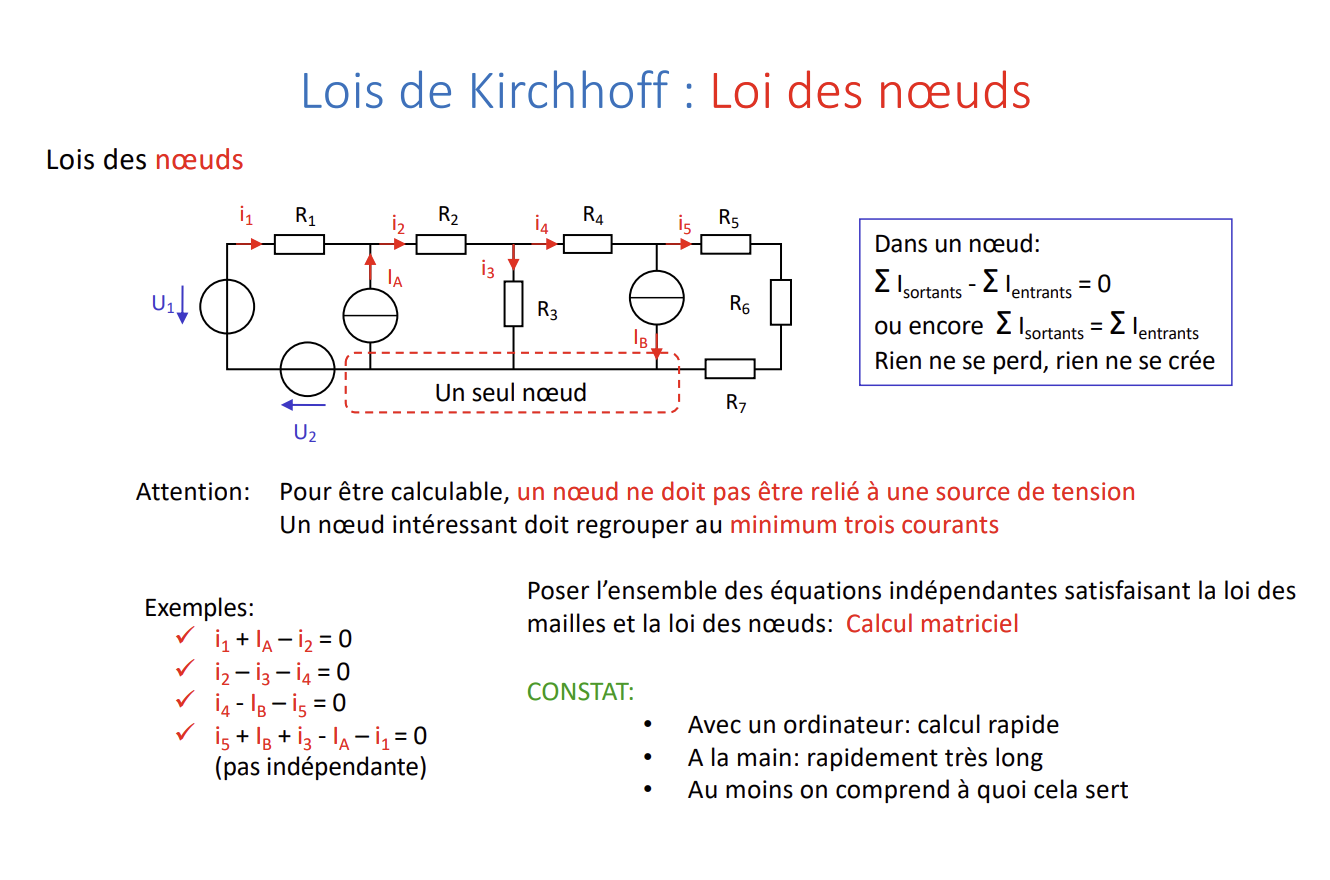
\includegraphics[
width=1.0\linewidth
]{../images/week03_08.png}

\end{center}


\begin{formula}

Dans un nœud :

\[
\sum I_{\text{sortants}} - \sum I_{\text{entrants}} = 0
\quad\text{ou encore}\quad
\sum I_{\text{sortants}} = \sum I_{\text{entrants}}
\]

Rien ne se perd, rien ne se crée.

où :

\begin{itemize}

\item $I_{\text{sortants}}$ : courants qui sortent du nœud [A] ;

\item $I_{\text{entrants}}$ : courants qui entrent dans le nœud [A].

\end{itemize}

\end{formula}


\begin{warning}

Pour être calculable, un nœud ne doit pas être relié à une source de tension.

Un nœud intéressant doit regrouper au minimum trois courants.

\end{warning}


\begin{important}

Poser l'ensemble des équations indépendantes satisfaisant la loi des mailles et la loi des nœuds : \textbf{calcul matriciel}.

\vspace{3pt}

\textbf{Constat :}

\begin{itemize}

\item avec un ordinateur : calcul rapide ;

\item à la main : rapidement très long ;

\item au moins on comprend à quoi cela sert.

\end{itemize}

\end{important}


%=========================================================
\section{Techniques de simplification : théorème de Millman}


Le théorème de Millman est issu des lois de Kirchhoff. Il permet de calculer une tension d'un nœud quelconque en fonction de son voisinage.

\begin{center}

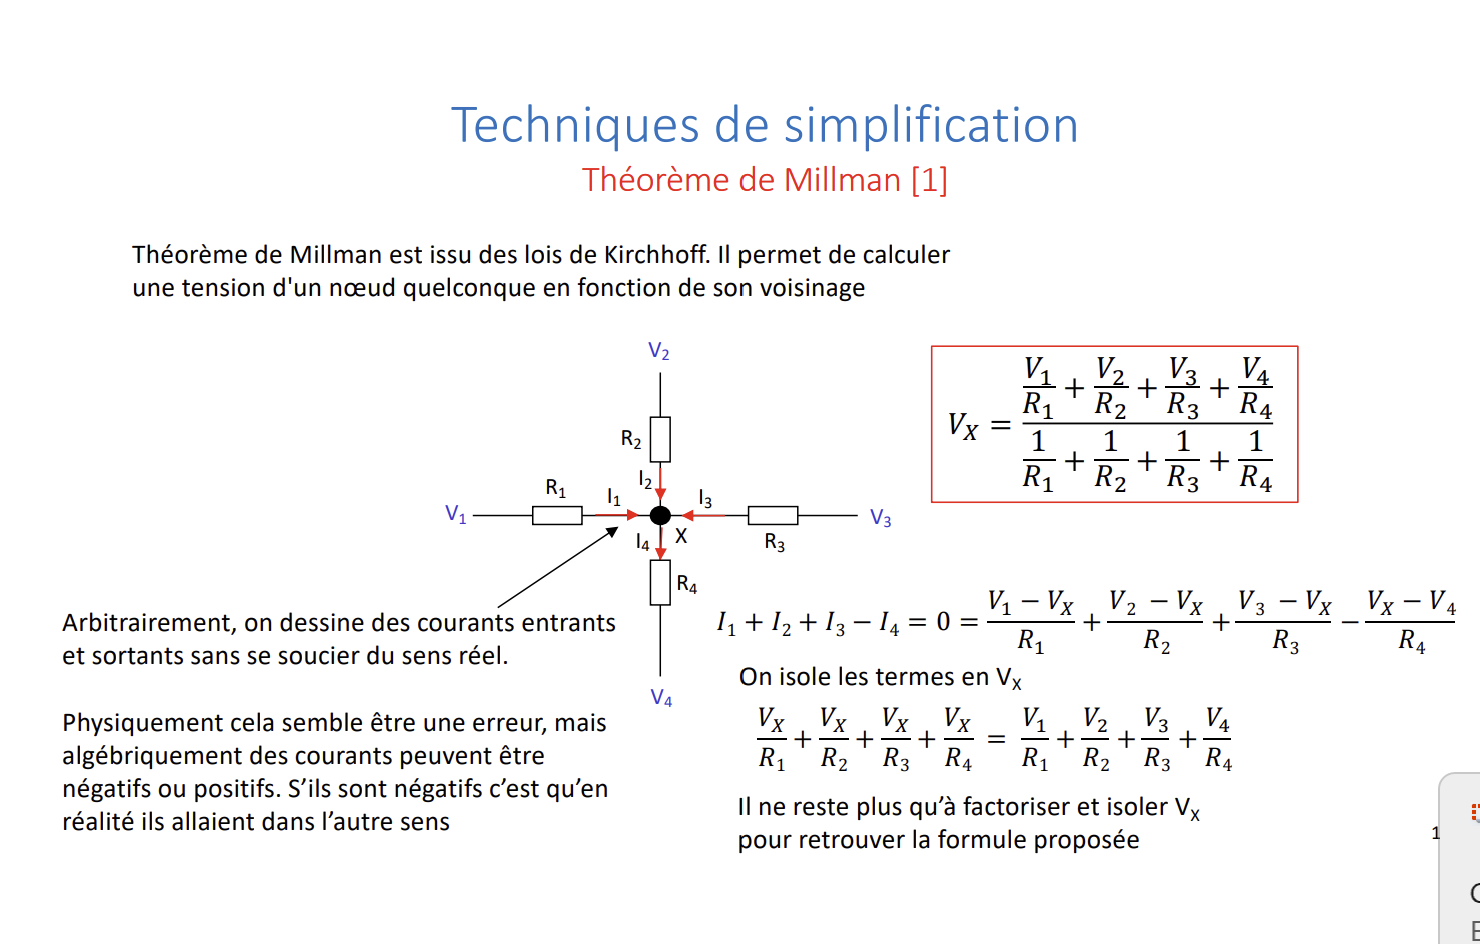
\includegraphics[
width=1.0\linewidth
]{../images/week03_09.png}

\end{center}

\begin{center}

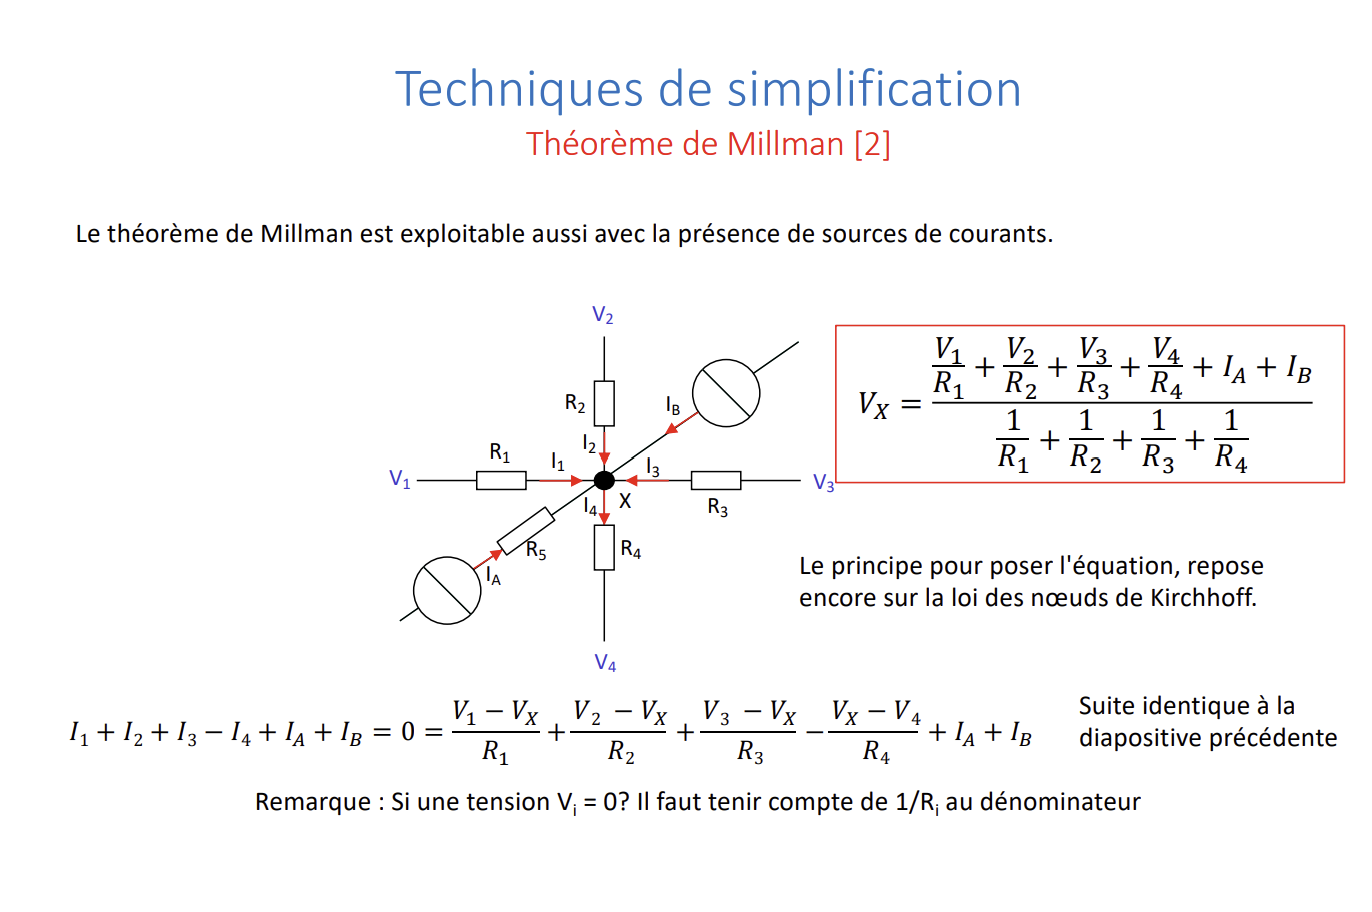
\includegraphics[
width=1.0\linewidth
]{../images/week03_10.png}

\end{center}


\begin{formula}

\[
V_X = \frac{\dfrac{V_1}{R_1} + \dfrac{V_2}{R_2} + \dfrac{V_3}{R_3} + \dfrac{V_4}{R_4} + I_A + I_B}{\dfrac{1}{R_1} + \dfrac{1}{R_2} + \dfrac{1}{R_3} + \dfrac{1}{R_4}}
\]

où :

\begin{itemize}

\item $V_X$ : potentiel du nœud $X$ cherché [V] ;

\item $V_k$ : potentiel connu à l'autre bout de la branche $k$ [V] ;

\item $R_k$ : résistance de la branche $k$ [$\Omega$] ; $1/R_k$ en [S] (siemens) ;

\item $V_k/R_k$ : un courant [A] ;

\item $I_A$, $I_B$ : courants des sources de courant qui \textbf{entrent} dans $X$ [A] (sans elles, on enlève $I_A + I_B$).

\end{itemize}

\end{formula}


\begin{important}

\textbf{Le problème}

On veut le potentiel $V_X$ d'un nœud $X$ relié par des résistances à des points dont on connaît le potentiel ($V_1$, $V_2$, \dots).

\vspace{3pt}

\textbf{Comment ça marche, en 4 étapes}

\begin{enumerate}[leftmargin=*,itemsep=1pt,topsep=1pt]

\item \textbf{On dessine les courants} de chaque branche, au hasard (entrants ou sortants) : un courant négatif veut juste dire qu'il va en réalité dans l'autre sens.

\item \textbf{Loi d'Ohm dans chaque branche} : la tension aux bornes de $R_k$ est $V_k - V_X$, donc le courant qui entre dans $X$ est $I_k = \frac{V_k - V_X}{R_k}$.

\item \textbf{Loi des nœuds en $X$} : la somme des courants entrants est nulle,
\[
\frac{V_1 - V_X}{R_1} + \frac{V_2 - V_X}{R_2} + \frac{V_3 - V_X}{R_3} - \frac{V_X - V_4}{R_4} = 0
\]

\item \textbf{On isole $V_X$} : on met les termes en $V_X$ d'un côté,
\[
V_X\left(\frac{1}{R_1} + \frac{1}{R_2} + \frac{1}{R_3} + \frac{1}{R_4}\right) = \frac{V_1}{R_1} + \frac{V_2}{R_2} + \frac{V_3}{R_3} + \frac{V_4}{R_4}
\]
puis on divise : on retrouve la formule.

\end{enumerate}

\textbf{L'intuition}

$V_X$ est une \textbf{moyenne pondérée} des potentiels voisins, avec des poids $1/R_k$ : plus une résistance est petite, plus son voisin \og tire \fg{} $V_X$ vers son potentiel.

\vspace{3pt}

\textbf{Avec des sources de courant}

Une source de courant impose son courant quel que soit $V_X$ : on ajoute juste son courant au numérateur ($+I_A$ s'il entre dans $X$, $-I_A$ s'il sort), et rien au dénominateur. La résistance $R_5$ en série avec la source n'apparaît pas : le courant est imposé de toute façon.

\vspace{3pt}

\textbf{Si un potentiel $V_i = 0$} (branche reliée à la masse) : le terme $V_i/R_i$ disparaît du numérateur, mais il faut \textbf{garder} $1/R_i$ au dénominateur.

\end{important}


\begin{example}

\textbf{1. Diviseur :} $V_1 = 10\,\text{V}$ par $R_1 = 1\,\text{k}\Omega$, et la masse ($V_2 = 0\,\text{V}$) par $R_2 = 1\,\text{k}\Omega$ :

\[
V_X = \frac{\frac{10}{1000} + 0}{\frac{1}{1000} + \frac{1}{1000}} = \frac{10\,\text{mA}}{2\,\text{mS}} = 5\,\text{V}
\]

\textbf{2. Trois branches :} $V_1 = 12\,\text{V}$, $R_1 = 2\,\text{k}\Omega$ ; $V_2 = 6\,\text{V}$, $R_2 = 1\,\text{k}\Omega$ ; masse ($V_3 = 0$), $R_3 = 2\,\text{k}\Omega$ :

\[
V_X = \frac{\frac{12}{2\text{k}} + \frac{6}{1\text{k}} + 0}{\frac{1}{2\text{k}} + \frac{1}{1\text{k}} + \frac{1}{2\text{k}}} = \frac{6 + 6 + 0\ \text{mA}}{0.5 + 1 + 0.5\ \text{mS}} = \frac{12\,\text{mA}}{2\,\text{mS}} = 6\,\text{V}
\]

Vérification par la loi des nœuds : $I_1 = \frac{12-6}{2\text{k}} = 3\,\text{mA}$, $I_2 = \frac{6-6}{1\text{k}} = 0$, $I_3 = \frac{0-6}{2\text{k}} = -3\,\text{mA}$ : la somme fait bien $0$.

\vspace{3pt}

\textbf{3. Avec une source de courant :} on reprend l'exemple 1 et on ajoute une source qui injecte $I_A = 5\,\text{mA}$ dans $X$ :

\[
V_X = \frac{10\,\text{mA} + 5\,\text{mA}}{2\,\text{mS}} = 7.5\,\text{V}
\]

\end{example}


%=========================================================
\section{Simplifications intermédiaires (résistances)}


\begin{center}

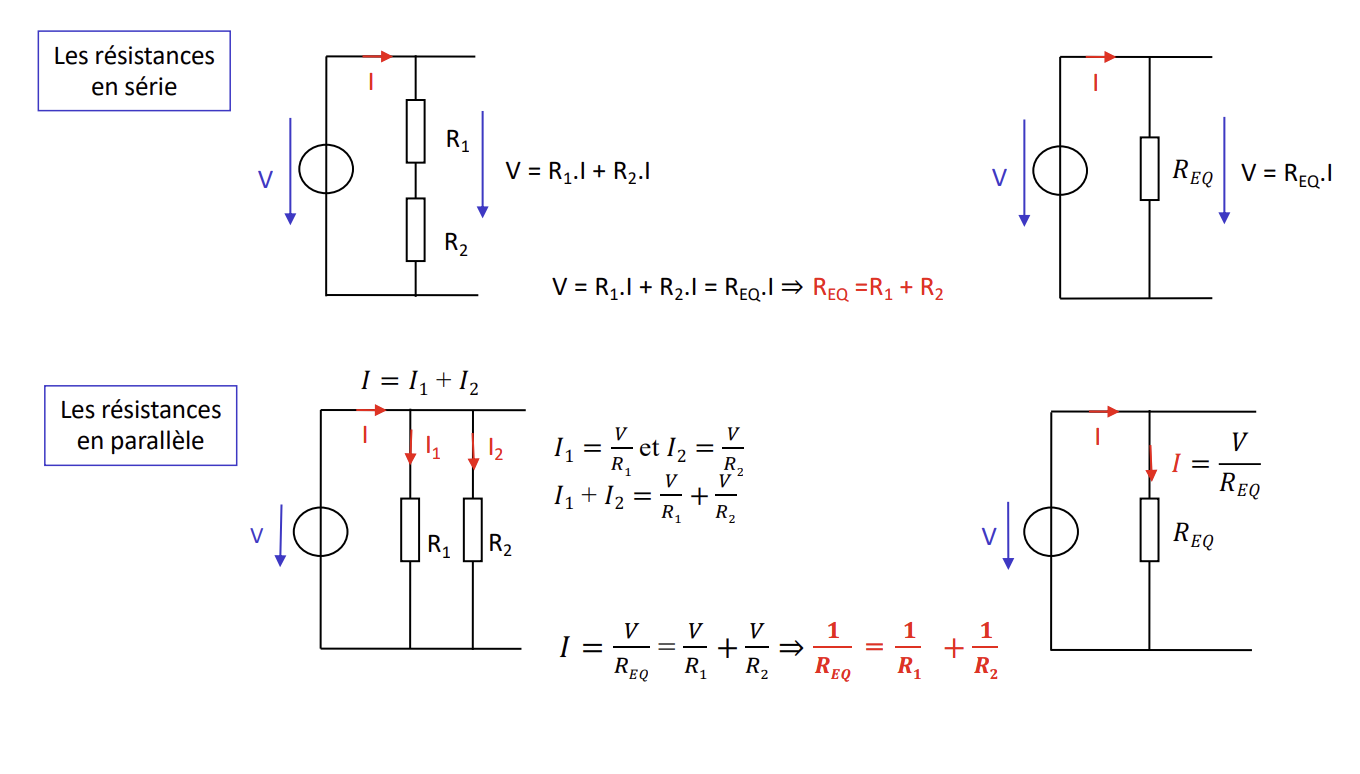
\includegraphics[
width=1.0\linewidth
]{../images/week03_11.png}

\end{center}


\begin{formula}

En série (même courant $I$) :

\[
V = R_1 I + R_2 I = R_{EQ} I
\quad\Rightarrow\quad
R_{EQ} = R_1 + R_2
\]

En parallèle (même tension $V$, $I = I_1 + I_2$) :

\[
I = \frac{V}{R_{EQ}} = \frac{V}{R_1} + \frac{V}{R_2}
\quad\Rightarrow\quad
\frac{1}{R_{EQ}} = \frac{1}{R_1} + \frac{1}{R_2}
\]

où :

\begin{itemize}

\item $R_1$, $R_2$ : résistances [$\Omega$] ; $R_{EQ}$ : résistance équivalente [$\Omega$] ;

\item $V$ : tension de la source [V] ;

\item $I$ : courant total [A] ; $I_1$, $I_2$ : courants dans $R_1$ et $R_2$ [A].

\end{itemize}

\end{formula}


%=========================================================
\section{Théorème de Kennelly}


Théorème de Kennelly : utile pour des transformations de structures en étoile vers triangle et réciproquement.

\begin{center}

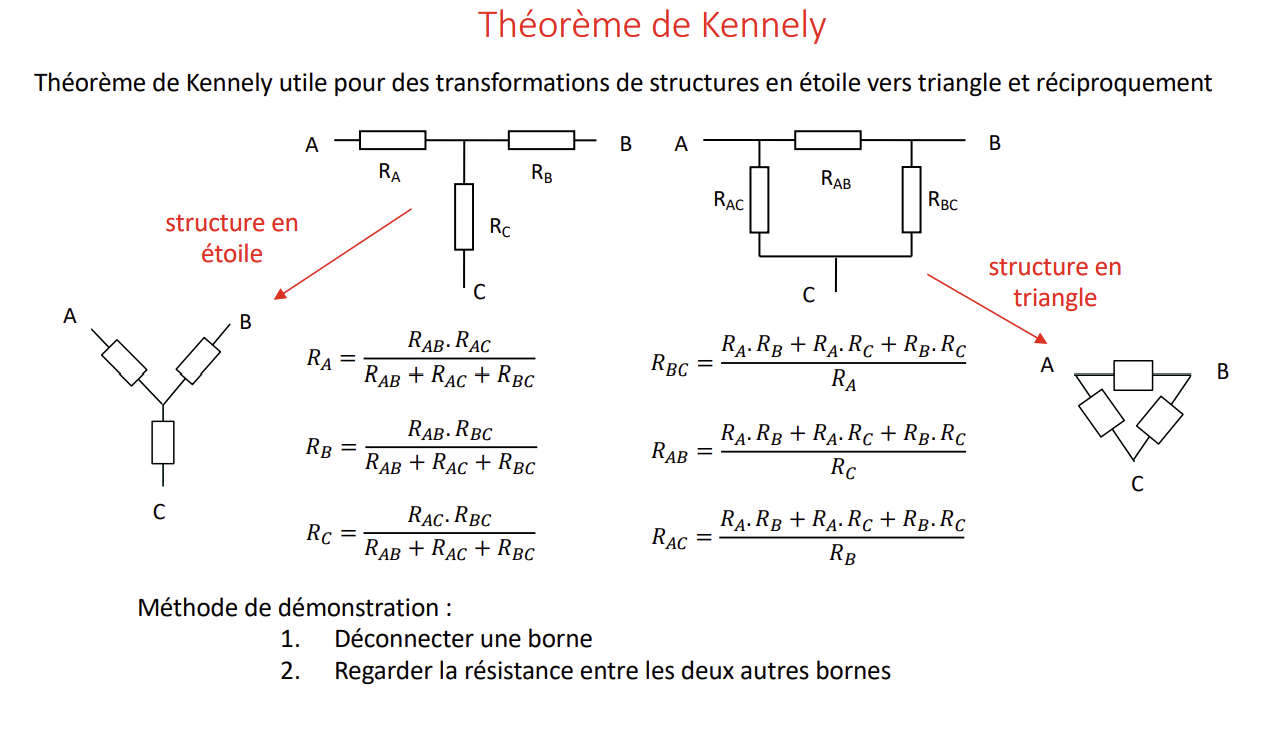
\includegraphics[
width=1.0\linewidth
]{../images/week03_12.png}

\end{center}


\begin{formula}

Triangle $\to$ étoile :

\[
R_A = \frac{R_{AB}\,R_{AC}}{R_{AB} + R_{AC} + R_{BC}}
\quad
R_B = \frac{R_{AB}\,R_{BC}}{R_{AB} + R_{AC} + R_{BC}}
\quad
R_C = \frac{R_{AC}\,R_{BC}}{R_{AB} + R_{AC} + R_{BC}}
\]

Étoile $\to$ triangle :

\[
R_{AB} = \frac{R_A R_B + R_A R_C + R_B R_C}{R_C}
\quad
R_{BC} = \frac{R_A R_B + R_A R_C + R_B R_C}{R_A}
\]
\[
R_{AC} = \frac{R_A R_B + R_A R_C + R_B R_C}{R_B}
\]

où :

\begin{itemize}

\item $A$, $B$, $C$ : les trois bornes de la structure ;

\item $R_A$, $R_B$, $R_C$ : résistances de l'étoile, chacune entre une borne et le centre [$\Omega$] ;

\item $R_{AB}$, $R_{BC}$, $R_{AC}$ : résistances du triangle, chacune entre deux bornes [$\Omega$].

\end{itemize}

\end{formula}


\begin{important}

\textbf{Le problème}

Certains circuits n'ont ni résistances en série, ni résistances en parallèle (comme le pont de l'exemple ci-dessous) : on ne peut rien fusionner, et il faudrait poser toutes les équations de Kirchhoff.

\vspace{3pt}

\textbf{L'idée}

Trois résistances reliant trois bornes $A$, $B$, $C$ peuvent être montées de deux façons :

\begin{itemize}

\item en \textbf{étoile} (ou en T) : chaque résistance va d'une borne à un point central commun ;

\item en \textbf{triangle} (ou en $\Pi$) : chaque résistance relie directement deux bornes.

\end{itemize}

Les deux sont \textbf{équivalentes} si, vues de l'extérieur, elles se comportent pareil : même résistance entre chaque paire de bornes. On peut alors remplacer l'une par l'autre sans rien changer au reste du circuit.

\vspace{3pt}

\textbf{Comment retenir les formules}

\begin{itemize}

\item Triangle $\to$ étoile : $R_A$ = produit des deux côtés du triangle qui touchent $A$, divisé par la somme des trois côtés.

\item Étoile $\to$ triangle : $R_{AB}$ = somme des produits deux à deux, divisée par la résistance de l'étoile \textbf{opposée} ($R_C$, celle qui ne touche ni $A$ ni $B$).

\end{itemize}

\textbf{Méthode de démonstration}

\begin{enumerate}[leftmargin=*,itemsep=1pt,topsep=1pt]

\item Déconnecter une borne (par exemple $C$, laissée en l'air).

\item Regarder la résistance entre les deux autres bornes :

\begin{itemize}

\item étoile : $R_A + R_B$ (en série, $R_C$ ne sert plus) ;

\item triangle : $R_{AB}$ en parallèle avec $(R_{AC} + R_{BC})$.

\end{itemize}

\item Les égaler, puis recommencer pour les deux autres bornes : 3 équations, 3 inconnues, on trouve les formules.

\end{enumerate}

\end{important}


\begin{example}

\textbf{Triangle de trois $3\,\text{k}\Omega$} :

\[
R_A = R_B = R_C = \frac{3\text{k}\cdot 3\text{k}}{3\text{k} + 3\text{k} + 3\text{k}} = 1\,\text{k}\Omega
\]

Et dans l'autre sens, une étoile de trois $1\,\text{k}\Omega$ donne $R_{AB} = \frac{1 + 1 + 1}{1}\,\text{k}\Omega = 3\,\text{k}\Omega$.

\end{example}


\textbf{Justification avec un exemple}

\begin{center}

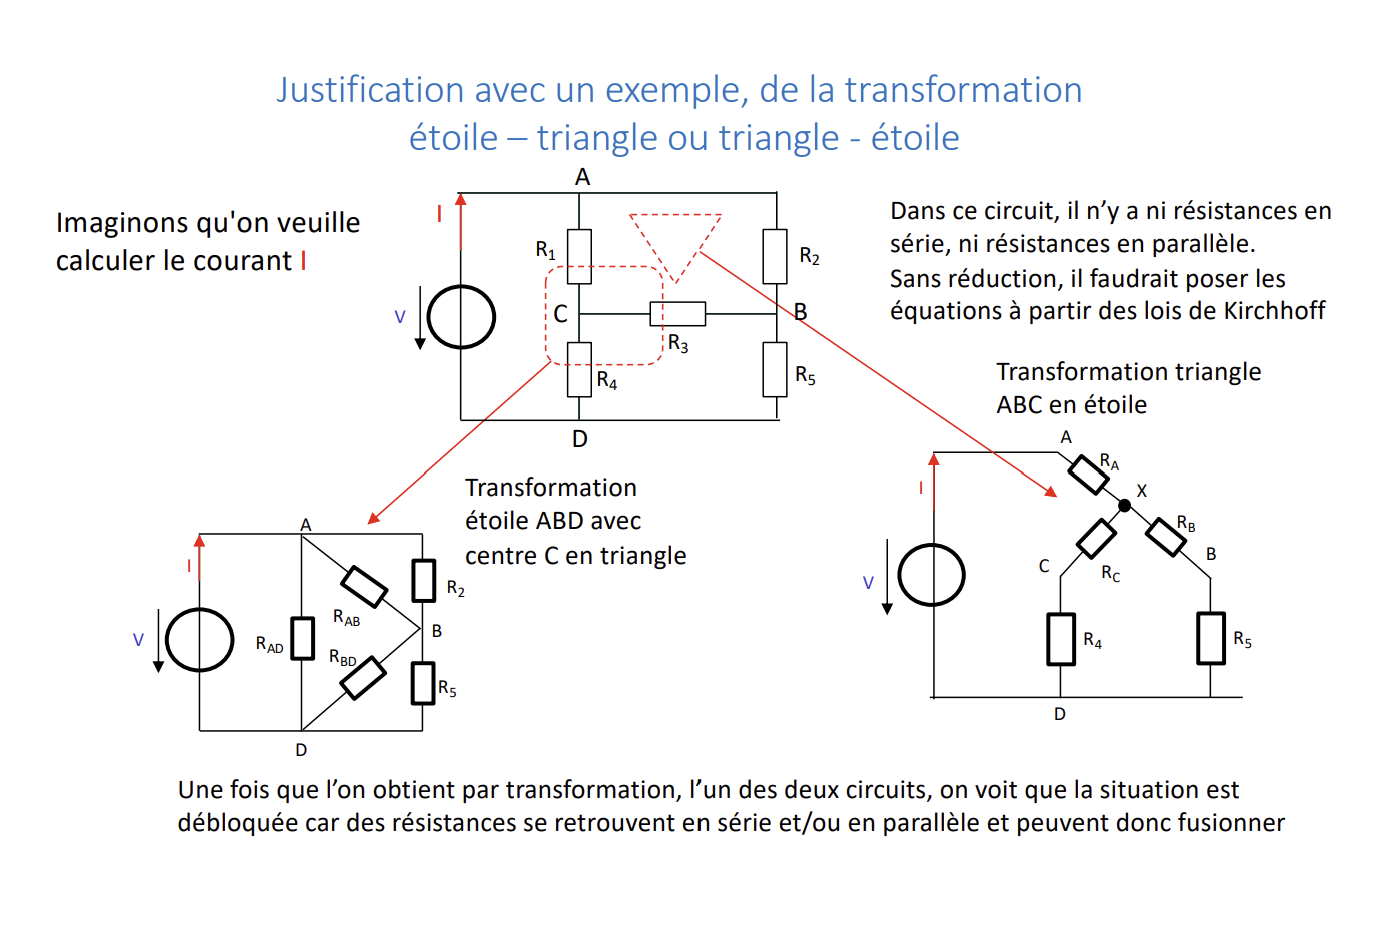
\includegraphics[
width=1.0\linewidth
]{../images/week03_13.png}

\end{center}

Imaginons qu'on veuille calculer le courant $I$. Dans ce circuit, il n'y a ni résistances en série, ni résistances en parallèle. Sans réduction, il faudrait poser les équations à partir des lois de Kirchhoff.

Une fois que l'on obtient par transformation l'un des deux circuits, on voit que la situation est débloquée, car des résistances se retrouvent en série et/ou en parallèle et peuvent donc fusionner.

\begin{example}

\textbf{Pas à pas (triangle $ABC$ en étoile, à droite) :}

\begin{enumerate}[leftmargin=*,itemsep=1pt,topsep=1pt]

\item On remplace le triangle $R_1$, $R_2$, $R_3$ par l'étoile $R_A$, $R_B$, $R_C$ de centre $X$.

\item $R_C$ et $R_4$ sont en série ; $R_B$ et $R_5$ aussi.

\item Ces deux branches relient $X$ à $D$ : elles sont en parallèle.

\item Le tout est en série avec $R_A$ :
\[
R_{EQ} = R_A + \frac{(R_C + R_4)(R_B + R_5)}{R_C + R_4 + R_B + R_5}
\qquad
I = \frac{V}{R_{EQ}}
\]

\end{enumerate}

\end{example}


%=========================================================
\section{Simplifications intermédiaires (les inductances)}


\begin{center}

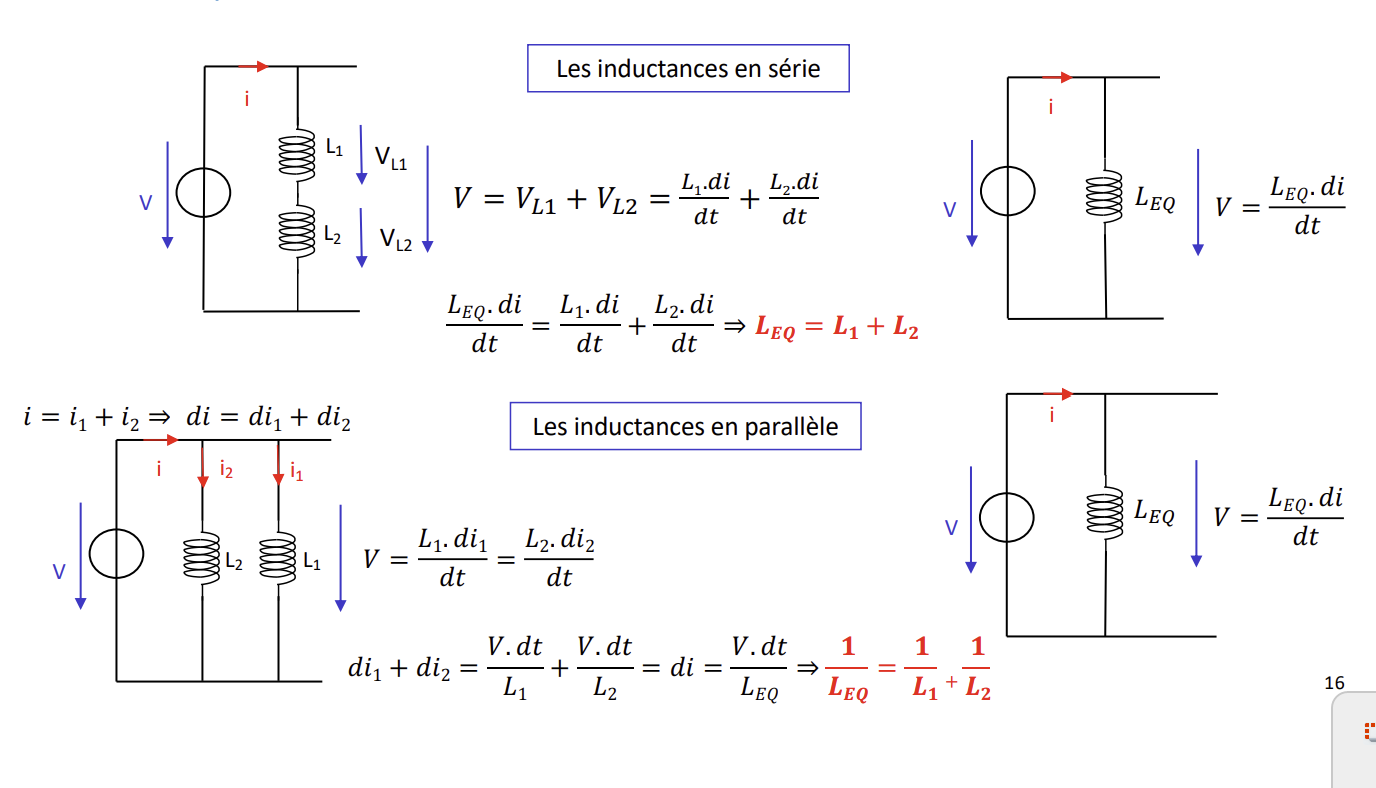
\includegraphics[
width=1.0\linewidth
]{../images/week03_14.png}

\end{center}


\begin{formula}

En série (même courant $i$, $V = V_{L1} + V_{L2}$) :

\[
\frac{L_{EQ}\,di}{dt} = \frac{L_1\,di}{dt} + \frac{L_2\,di}{dt}
\quad\Rightarrow\quad
L_{EQ} = L_1 + L_2
\]

En parallèle (même tension $V$, $i = i_1 + i_2$ donc $di = di_1 + di_2$) :

\[
di_1 + di_2 = \frac{V\,dt}{L_1} + \frac{V\,dt}{L_2} = di = \frac{V\,dt}{L_{EQ}}
\quad\Rightarrow\quad
\frac{1}{L_{EQ}} = \frac{1}{L_1} + \frac{1}{L_2}
\]

où :

\begin{itemize}

\item $L_1$, $L_2$ : inductances [H] ; $L_{EQ}$ : inductance équivalente [H] ;

\item $V$ : tension de la source [V] ; $V_{L1}$, $V_{L2}$ : tensions aux bornes de $L_1$, $L_2$ [V] ;

\item $i$ : courant total [A] ; $i_1$, $i_2$ : courants dans $L_1$, $L_2$ [A] ;

\item $di$, $dt$ : petites variations du courant [A] et du temps [s].

\end{itemize}

\end{formula}


%=========================================================
\section{Simplifications intermédiaires (capacités parallèles)}


\begin{center}

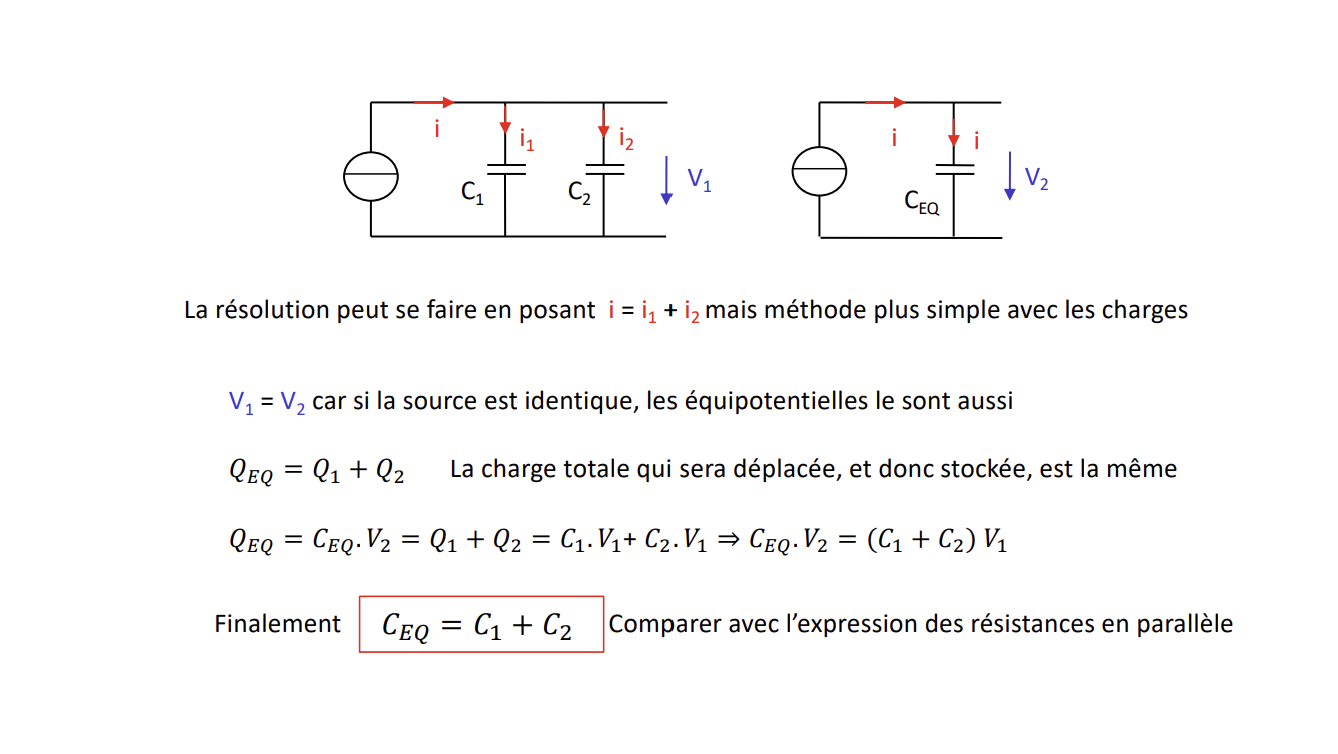
\includegraphics[
width=1.0\linewidth
]{../images/week03_15.png}

\end{center}

La résolution peut se faire en posant $i = i_1 + i_2$, mais la méthode est plus simple avec les charges.

\begin{formula}

$V_1 = V_2$ car si la source est identique, les équipotentielles le sont aussi.

\[
Q_{EQ} = Q_1 + Q_2
\]

La charge totale qui sera déplacée, et donc stockée, est la même.

\[
Q_{EQ} = C_{EQ}\,V_2 = Q_1 + Q_2 = C_1 V_1 + C_2 V_1
\quad\Rightarrow\quad
C_{EQ}\,V_2 = (C_1 + C_2)\,V_1
\]

Finalement :

\[
\boxed{C_{EQ} = C_1 + C_2}
\]

(à comparer avec l'expression des résistances en parallèle).

où :

\begin{itemize}

\item $C_1$, $C_2$ : capacités [F] ; $C_{EQ}$ : capacité équivalente [F] ;

\item $Q_1$, $Q_2$, $Q_{EQ}$ : charges stockées [C] ;

\item $V_1$, $V_2$ : tensions aux bornes [V] ;

\item $i$, $i_1$, $i_2$ : courants [A].

\end{itemize}

\end{formula}


\end{multicols}

\end{document}
